\documentclass[../../../analisi-dei-requisiti.tex]{subfiles}

\begin{document}

\subsubsection{AUC16: Eliminazione visualizzatore}%
\label{subs:AUC16}

\begin{figure}[H]
  \centering
  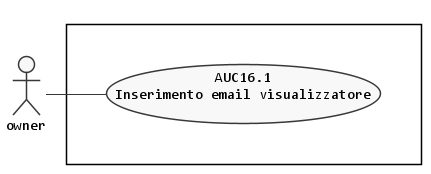
\includegraphics[width=100mm]{eliminazione-visualizzatore.png}
  \caption{AUC16: Eliminazione visualizzatore}%
  \label{fig:AUC16}
\end{figure}

\begin{description}
  \item[Codice:] AUC16;
  \item[Titolo:] Eliminazione visualizzatore;
  \item[Attori primari:] owner;
  \item[Precondizione:] il sistema deve rendere disponibile la pagina di eliminazione visualizzatore;
  \item[Postcondizione:] l'utente non è più visualizzatore;
  \item[Scenario principale:]
        \begin{enumerate}
          \item l'owner vuole eliminare i privilegi ad un utente visualizzatore.
        \end{enumerate}
\end{description}

\subsubsection{AUC16.1: Inserimento email visualizzatore}%
\label{subs:AUC16.1}
\begin{description}
  \item[Codice:] AUC16.1;
  \item[Titolo:] Inserimento email visualizzatore;
  \item[Attori primari:] owner;
  \item[Precondizione:] il sistema deve rendere disponibile la possibilità di inserire l'email del visualizzatore da eliminare;
  \item[Postcondizione:] l'email viene opportunamente inserita;
  \item[Scenario principale:]
        \begin{enumerate}
          \item l'owner inserisce l'email del visualizzatore da eliminare.
        \end{enumerate}
\end{description}

\end{document}
